\documentclass[11pt]{amsart}
\usepackage{color}
\usepackage{color}
\usepackage{tikz}
\usetikzlibrary{decorations.markings, hobby, knots}
\usepackage{pgffor}

\begin{document}

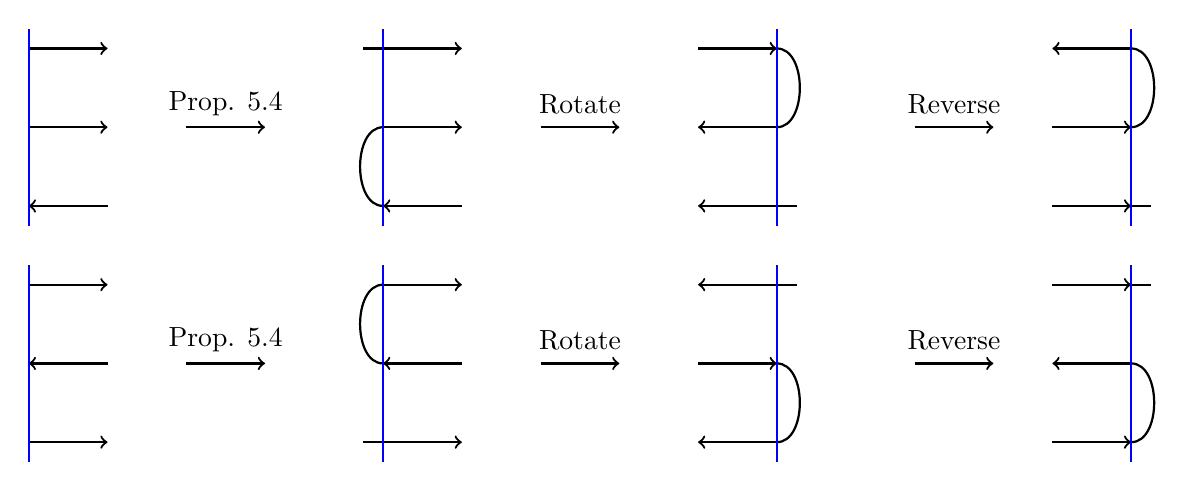
\begin{tikzpicture}[thick]
%First Row
% Orientations

\draw[<-] (0,0) -- (1,0);
\draw[->] (0,1) -- (1,1);
\draw[->] (0,2) -- (1,2);
\draw[blue] (0,2.25) -- (0,-0.25);

\draw[->] (2,1) -- (3,1);
\draw (2.5,1.3) node{Prop. 5.4};

%After cobordism
\begin{scope}[xshift = 4.5cm]
\draw[<-] (0,0) -- (1,0);
\draw[->] (0,1) -- (1,1);
\draw[->] (0,2) -- (1,2);
\draw (0,0) to [out = 180, in = 180] (0,1);
\draw (-.25,2) to (0,2);
\draw[blue] (0,2.25) -- (0,-0.25);
\draw[->] (2,1) -- (3,1);
\draw (2.5,1.3) node{Rotate};
\end{scope}

%After rotating

\begin{scope}[xshift = 8.5 cm]
    \draw[<-] (0,0) -- (1.25,0);
    \draw[<-] (0,1) -- (1,1);
    \draw[->] (0,2) -- (1,2);
    \draw (1,2) to [out = 0, in = 0] (1,1);
    \draw[blue] (1,2.25) -- (1,-0.25);

    \draw[->] (2.75,1) -- (3.75,1);
    \draw (3.25,1.3) node{Reverse};

\end{scope}

%After reversing

\begin{scope}[xshift = 13 cm]
    \draw[->] (0,0) -- (1,0);
    \draw (1,0) -- (1.25,0);
    \draw[->] (0,1) -- (1,1);
    \draw[<-] (0,2) -- (1,2);
    \draw (1,2) to [out = 0, in = 0] (1,1);
    \draw[blue] (1,2.25) -- (1,-0.25);

\end{scope}

% 2nd Row

\begin{scope}[yshift = -3cm]
% Orientations

\draw[->] (0,0) -- (1,0);
\draw[<-] (0,1) -- (1,1);
\draw[->] (0,2) -- (1,2);
\draw[blue] (0,2.25) -- (0,-0.25);

\draw[->] (2,1) -- (3,1);
\draw (2.5,1.3) node{Prop. 5.4};

%After cobordism
\begin{scope}[xshift = 4.5cm]
\draw[->] (0,0) -- (1,0);
\draw[<-] (0,1) -- (1,1);
\draw[->] (0,2) -- (1,2);
\draw (0,1) to [out = 180, in = 180] (0,2);
\draw (-.25,0) to (0,0);
\draw[blue] (0,2.25) -- (0,-0.25);
\draw[->] (2,1) -- (3,1);
\draw (2.5,1.3) node{Rotate};
\end{scope}

%After rotating

\begin{scope}[xshift = 8.5 cm]
    \draw[<-] (0,0) -- (1,0);
    \draw[->] (0,1) -- (1,1);
    \draw[<-] (0,2) -- (1.25,2);
    \draw (1,0) to [out = 0, in = 0] (1,1);
    \draw[blue] (1,2.25) -- (1,-0.25);

    \draw[->] (2.75,1) -- (3.75,1);
    \draw (3.25,1.3) node{Reverse};

\end{scope}

%After reversing

\begin{scope}[xshift = 13 cm]
     \draw[->] (0,0) -- (1,0);
    \draw[<-] (0,1) -- (1,1);
    \draw[->] (0,2) -- (1,2);
    \draw (1,2) -- (1.25,2);
    \draw (1,0) to [out = 0, in = 0] (1,1);
    \draw[blue] (1,2.25) -- (1,-0.25);

    \draw[blue] (1,2.25) -- (1,-0.25);

\end{scope} 
\end{scope}


    
\end{tikzpicture}

\end{document}